%Your introduction should describe your product concept in sufficient detail that the architectural design will be easy to follow. The introduction may include information used in the first sections of your SRS for this purpose. At a minimum, ensure that the product concept, scope and key requirements are described.
\quad \quad Cerberus, is a wireless wrist module system that notifies deaf or hard of hearing individuals of events happening around them. The Cerberus system must be used in conjunction with the Ring system. It will not work without access to a Ring system. The wearer will be notified by the wrist module from a vibration. The vibration signals them to check their phone to see the event description of what triggered the vibration. The event notification will be displayed through the Cerberus phone app. The Cerberus phone app will receive notifications from the server. The server will communicate with the Ring system and push event notifications from the Ring system to the phone app. Events from the Ring system will include the doorbell being rung, the motion detector being tripped, or the alarm system going off.

\quad The Cerberus system includes the wrist module, the app, and the server. The wristband will include a vibration module to notify the wearer. It will also include LED lights to notify the wearer of the noise level around them. The wristband will be wireless and chargeable. Inside the wristband it will have a Bluetooth module to connect to the phone app. Users will need to make an account on the phone app in order to use it. On the phone app, the user will able to see present and past notifications. Users will also be able to change settings like turning on silent mode or change vibration patterns for the wristband. The Cerberus server will connect the phone and Ring system together. It will forward notifications from the Ring system to the app. It will also host a database with our users' account information and settings. 

\begin{figure}[h!]
	\centering
   	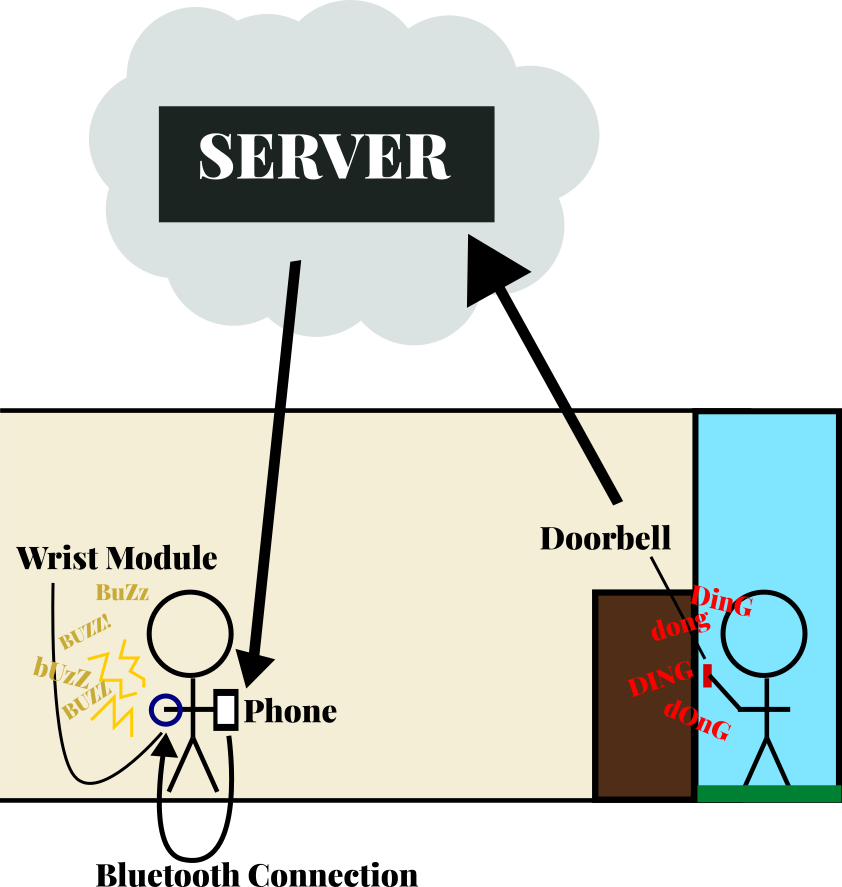
\includegraphics[width=0.60\textwidth]{images/high-level-system-overview.png}
    \caption{Conceptual drawing}
\end{figure}